\documentclass[10pt,a4paper]{article}
\usepackage[driver=xetex,a4paper]{geometry} % propper margins on a4 paper
\usepackage{pdfpages} % to include cover
\usepackage{url}
\usepackage[hidelinks]{hyperref} % make contents and references clickable in pdf
\usepackage{multicol} % allows multiple colums
\usepackage{titlesec} % adjust whitespace around headings and improves placing
\usepackage{microtype} % adjusts kerning and letterspacing
\usepackage{soul} %striketrough
\usepackage{parskip} % newline instead of indenting
\usepackage{graphicx} % include images

\usepackage{fontspec} % allows custom fonts
\setmainfont[BoldFont=Source Sans Pro Bold,AutoFakeSlant=0.3]{Source Serif Pro}
\setmonofont{Source Code Pro}

\usepackage{listings} % allows code listings
\usepackage{lstautogobble}
\lstset{basicstyle=\footnotesize\ttfamily,
        breaklines=true,
        keepspaces=true,
        xleftmargin=6pt,
        %gobble=2, % ignore first 2 spaces indents in code listings
        autogobble,
        captionpos=b,
        morekeywords={Func,Data,TypeFunc,Module,TypeAlias,Inherit,is},
        keywordstyle=\bfseries,
        escapeinside=\#\# } % non ASCII-characters won't render properly. Use #\verb|contents|#

\lstnewenvironment{code}[1][]{% make code unsplittable
   \noindent
   \minipage{\linewidth} 
   \lstset{#1}}
   {\endminipage}

\usepackage[sorting=none,backend=biber]{biblatex} %citations
\addbibresource{references.bib}
\renewcommand*{\bibfont}{\small} % small references at the end

\usepackage{draftwatermark}
\SetWatermarkFontSize{40pt}
\SetWatermarkLightness{0.8}
\SetWatermarkAngle{0}
\SetWatermarkVerCenter{5em}

\begin{document}
% disable page numbers
\pagestyle{empty} 

% cover page

\includepdf[pages=1]{cover.pdf}
\newpage

% start page numbers
\setcounter{page}{1}
\pagenumbering{arabic}
\pagestyle{plain}

% actual document

\begin{multicols}{2}
\tableofcontents
\end{multicols}
\pagebreak

\begin{multicols}{2}

\section*{Abstract}
This project is about the development of the back-end of the bootstrap compiler for the Meta Casanova 3 language.
The back-end is responsible for generating an executable after receiving the type-checked program representation from the front-end.
In this thesis, we will walk through the back-end and examine the various parts and their design decisions.
In this way, this document aims to be useful to the future developers of the back-end.

\section{Introduction}
Games are difficult to develop~\cite{blow}.
To make writing games easier, a new language was developed: Casanova.

Implementing the Casanova compiler proved difficult.
Compilers are complex programs that have to operate on a wide range of inputs.
Since compilers have such a large input-space, the chance of a bug hiding somewhere is substantial. 
But for al their complexity, compilers also have to be bug-free since every program can only be as bug-free as its compiler~\cite{thompson}.

Abstractions can help in this regard.
The limits of which were observed when implementing the compiler for the Casanova language in F\#.
The compiler was 1480 lines long, and became unmaintainable.
After a rewrite in MC it was 300 lines~\cite{maggiore}.

The primary reason for this was the lack of higher-order type operators.
Higher-order type operators made abstractions such as monad-transformers impossible, hampering modularity and resulted in a lot of non-reusable boilerplate code~\cite{pierce}.

\subsubsection{Structure}
We will first discuss the context of the assignment in section~\ref{context}.
Then we will give a short overview of Meta Casanova in section~\ref{metacasanova}.

Section~\ref{research}, the main part of is thesis, is next.
It presents the main research question and splits it in sub-questions.
Each sub-question is then answered in each subsection.

Section~\ref{results} presents the evidence that the requirements of the main research question have been met.
This is followed by conclusions in section~\ref{conclusions} that summarize the results.
After the thesis proper, we give recommendations for the future development of the back-end in section~\ref{recommendations}.
Section~\ref{evaluation} is the last part of the thesis, and shows that the Dublin descriptors have been met.

%The appendices contain the contact details of the stakeholders, a glossary and the full source code of the back-end.
{The source code is available in online\protect\footnote{in \url{Sources/Mark III/Interpreter BasicMetacasanova/} at \url{https://github.com/vs-team/metacompiler}}}.

\subsection{Output language}
The first research question had the most impact on the project, and was one that was difficult to change later on.

\textit{In what programming language should the code-generator produce its output?}

This may be different than the language the code-generator is written in.
The code-generator is written in F\#, like the rest of the compiler.
The reason we use F\#, rather than Meta-Casanova 2, is because Meta Casanova 2 lacks tool support, such as descriptive error messages and debuggers.

\subsubsection{Unmanaged languages}
Since speed was one of the requirements, I first looked at solutions with unmanaged parts.
Unmanaged code is code that is not interpreted by a runtime, but is instead executed directly.
%It is also much less restrictive than the .NET runtime because the .NET bytecode is strongly typed.\cite{ecma335}

The main advantage of unmanaged code is that the fast LLVM code generator can be used.
LLVM is a ``collection of modular and reusable compiler and toolchain technologies.''\cite{llvm}
Specifically, the LLVM optimizer is valuable.
It is used in the Clang, a C/C++ compiler on par with gcc, and with little effort can be use it to optimize our generated code.
This would mean we get all the optimisations of LLVM with relative ease.
It would however mean that we had to implement a garbage collector, as LLVM does not come with one.
 
.NET compatibility is also required, as explained in section \ref{whydotnet}.
There are a few systems that allow for managed and unmanaged code to communicate.
The most viable are P/invoke, C++/CLI interop, and a hosted runtime.

\paragraph{P/invoke}
Platform Invocation Services allows managed code to call unmanaged functions that are implemented in a DLL.\cite{msdn_pinvoke}

This is the most common form of inter-op, and has great documentation.
However, there are two big disadvantages.

\begin{enumerate}
    \item .NET can only call native functions, not the other way around.
        This means that the bulk of the control flow happens inside .NET, minimizing the fast native code.
    \item Transfering data between .NET and native code has a high performance cost\cite{msdn_interop_performance}, since it has to be serialized.
        This overhead is so large that we expect it to negate any performance benefit from using native code.
\end{enumerate}

Because of this, P/Invoke was not chosen.

\paragraph{C++/CLI}
C++ for the Common Language Infrastructure is a programming language designed for interoperability with unmanaged code.\cite{msdn_c++cli}

While it seems like it does exactly what we need, it has portability issues.
The only C++/CLI compiler runs on windows and it only compiles for processors with the x86 architecture\cite{mono_c++cli}.
Besides that, non-typesafe operations (the main advantage of C++/CLI) are only allowed on windows.\cite{mono_c++cli}

This means C++/CLI is not cross-platform enough.

\paragraph{Hosted runtime}
It is possible to embed a .NET runtime inside a native program.
This would make it so the control flow takes place inside the native part.

This seems like the best solution out of the native hybrids.
However it still has two drawbacks.
The mono runtime has a different interface than the microsoft .NET api, leading to incompatible programs \cite{mono_embedding}.
The same large serialization overhead as P/Invoke is present\cite{msdn_hosted}.

\subsubsection{.NET languages}
None of the inter-op methods offer a satisfactory solution.
They all have downsides that outweigh the benefits.
It was decided to let go of the LLVM code-generation in favor of a more portable and reliable system.

Stability is a big advantage because everything happends inside the .NET runtime.
This has a higher chance of working on non-native platforms than the hybrid solutions.

\paragraph{F\#} is a functional/declarative language in the .Net family\cite[fsharp].
It would be a natural choice, since the compiler is written in it.
However, it is quite slow\cite{fsharp_slow} and resists the imperative style of the generated code.
The programmer has also less control of the program execution, as F\# is a more higher-level language\cite{fsharp}

A version of the code generator was made that used F\#, but it proved too cumbersome since there was no mechanism to simply skip rules if they failed.

% maybe look for Mohammeds compiler written in F#?

\paragraph{C\#}
is an imperative, object-oriented language\cite{csharp}.
It is the most popular .NET language\cite{Meyerovich}, so the compiler gets the most attention by Microsoft.
It is also easy to debug, as it has the most mature debugging tools.

When implementing the code-generator in this style, it was possible to write the code-generator so that the output-code is straight-line code.
This is opposed to F\#, where I had to generate a tree-structure as an output.
This greatly improved debugability and simplicity of implementation.

\paragraph{CIL}
(Common Intermediate Language) is the bytecode that all the languages are compiled to.
Since it is typed, it has the same restrictions as C\#.[source]
As a result, it makes debugging and verification harder, with little to no gain.
It also ommits the optimizations of the C\# compiler, such as dead-code elimination and stuff\cite{csharp_optimizations}.

\subsubsection{Conclusion}
The debugability together with a lot of control make C\# the best choice for code generation.


\section{Meta Casanova}
It is necessary to understand a subset of Meta Casanova(MC) in order to understand the problem-space.
This section will cover the subset of the language that is relevant for code-generation.

Meta Casanova is a functional, declarative language.
It allows for multiple implementations of functions called \textit{rules}.
Rules may fail, in that case the next rule will be attempted.
This will continue until a rule succeeds, or no rule matches in which case the program throws an exception.

\subsection{Data}\label{mcdata}
\texttt{Data} declarations declare a discriminated union.\cite{algebraic_datastructures}.

\begin{MC}
Data "nil" -> list<'a>
Data 'a -> "::" -> list<'a> -> list<'a>
\end{MC}

It defines the same structure as this F\#-like pseudocode.

\begin{FS}
List<'a> = nil 
         | 'a :: List<'a>
\end{FS}

In this example, the list type is declared with two constructors.
They specify that a lists can be constructed in two ways: with \verb|nil| and with \verb|::| surrounded with a term of type \verb|'a|, and a term of type \verb|list<'a>|.

Conversely, they also specify that an list can be destructed in two ways.
The programmer will assert which destructor is expected, and the rule fails if the destructor does not match.
An example of this is shown later, in subsection ``Funcs''.

Additionally, constructors may be manipulated and partially applied like functions.
This allows for greater flexibility at the cost that function and constructor names need to be unique in their namespace.

%\subsection{Polymorphism}
%Polymorphic data structures are supported with the \textbf{\texttt{is}} keyword.
%
%\begin{code}
%Data "error" -> string -> failableList<'a>
%failableList 'a is list<'a>
%\end{code}
%
%\noindent
%This means every constructor of the \verb|list| is also a valid constructor of \verb|failableList|, but not vice-versa.

\subsection{Funcs}
Func declarations specify a new function and its type.

\begin{MC}
Func "length" -> list<'a> -> int
\end{MC}

As with constructors, functions may be freely manipulated and partially applied, and have the restriction that their name must be unique in their namespace.

\subsection{Rules}
Meta-Casanova uses a syntax similar to that of natural deduction.
For each Func declaration, there are one or more rules that define it.

\begin{MC}
---------------
length nil -> 0

length xs -> res
---------------------
length x::xs -> 1+res
\end{MC}

A rule is comprised of a line with below it on the left of the arrow the input, and on the right the output.
The statements above the horizontal line are called \textit{premises}\label{premises}.
They can be assignments like in the example above, or conditionals like \verb|a==b| or \verb|c<d|.

In the case of assignments, they create a \textit{local identifier}.
These identifiers are local to the rule they appear in.
The input arguments of the rule are also local identifiers.

We can now call the function \verb|length| with an example list:

\begin{MC}
  1::(2::nil) -> x
  length x    -> res
\end{MC}

The first premise constructs a list called ``x'', and the second statement calls length with that list.
The program will execute as follows:

\begin{MC}[escapeinside=\#\#]
length 1::(2::nil)
    #\st{nil}#
    x::xs → 1+(length 2::nil)
        #\st{nil}#
        x::xs → 1+(length nil)
            nil → 0
            #\st{x::xs}#
\end{MC}

After which the function stops calling itself and starts accumulating the result on the way down.

\begin{MC}[gobble=2]
          1 ← 1+0
      2 ← 1+1
  2
\end{MC}

After which it tells us correctly that the length of the list 1::(2::nil) is indeed 2.

\subsection{Main}
Each program needs an entry point.
The entry point of an MC program is the main function.

\begin{MC}
    length 1::(2::nil) -> res
    -------------------------
    main -> res
\end{MC}

The results of the main function are printed on the console.
The previous program would therefore print \verb|2| on the screen.


TODO: metacasanova type syntax
TODO: metacasanova no longer matches multiple statements
\subsection{The front-end interface}
The second research question is about the specification of the front-end interface.

\textit{What should the interface between the front-end and the back-end be?}

The front-end interface contains all the input for the backend.
This makes testing very easy, as the rest of the backend only relies on its input.

\subsubsection{Interface}
The interface is all contained in a single datastructure.

\begin{FS}
type Interface = {
  datas      : List<Id*Data>
  funcs      : List<Id*List<rule>>
  lambdas    : List<LambdaId*rule>
  main       : rule
  flags      : CompilerFlags
  assemblies : List<string> 
}
\end{FS}

As you can see, the interface contains the data declarations, function definitions, lambda definitions and a main function.

The design principles for this interface were simplicity and minimalism.
There should be as few ways as possible to represent the same program.
This makes testing easier and minimizes bugs that appear only in certain representations of the same program.

All the symbols in the descriptions are provided with monomorphic types by the front-end.
Functions with generic types are made concrete by the front-end.

The reason that \texttt{datas}, \texttt{funcs} and \texttt{lambdas} are defined as a list of key-value pairs instead of as a Map, is that the keys are not guaranteed to be unique.
Since MC allows polymorphic types, one indentifier may be defined multiple times: once for each type.
There is no performance penalty for the back-end, as no lookups by identifier are performed.

\subsubsection{Data declarations}
The data declarations are grouped with the identifier of the constructor.

\begin{FS}
datas : List<Id*Data>
\end{FS}

Where \verb|Data| is simply a list of input types and output types.

\begin{FS}
type Data = {
  args       : List<Type>
  outputType : Type
}
\end{FS}

Where \verb|Type| represents a monomorphic MC type.

%\begin{FS}
%type Type 
%  = DotNetType      of TypeId
%  | McType          of TypeId
%  | TypeApplication of Type*List<Type>
%  | Arrow           of Type*Type
%\end{FS}

We can illustrate this by defining a tuple an a union in MC.

\begin{MC}
Data int -> "," -> string -> Tupple<int string>
Data "fst" -> int    -> Union<int string>
Data "snd" -> string -> Union<int string>
\end{MC}

This will appear as the following list in the interface:

{\footnotesize
\begin{tabular}{lll}
    \textbf{\normalsize identifier} & \textbf{\normalsize arguments} & \textbf{\normalsize type}\\
    \verb:",":   & \verb:int:; \verb:string: & \verb:Tuple<int string>: \\
    \verb:"fst": & \verb:int:                & \verb:Union<int string>: \\
    \verb:"snd": & \verb:string:             & \verb:Union<int string>: \\
\end{tabular}
}


\subsubsection{Rule containers}

Function and lambda definitions, as well as the main function contain rules.

\begin{FS}
  funcs   : List<Id*List<rule>>
  lambdas : List<LambdaId*rule>
  main    : rule
\end{FS}

Functions in MC can contain multiple rules that implement them.

The entry point of the program is defined by a single rule, here called \verb|main|.
It is not a full function since full functions can have multiple rules.
This was done to make the entry-point as simple as possible.

\subsubsection{Rules}

Functions are defined with of one or more \textit{rules}.
This is how they are represented in the interface.

\begin{FS}
type rule = {
  premises    : List<premise*linenr>
  input       : List<local_id>
  output      : local_id
  typemap     : Map<local_id,Type>
  declaration : Position
  definition  : Position
}
\end{FS}

The main component of rules is its premises.
These are the instructions that make up the rule.
The instruction set is described in section~\ref{ir}.

The premise list also contains line numbers for each premisse.
This is debug information, that is used by the embedded debugger\footnote{see section~\ref{debugger}}.

Next are the inputs and output of the rule.
Input and outputs consist only of local identifiers.
This is because of \textit{normalization}\footnote{see section~\ref{normalization}}.

In the case that a rule-input or output has an expression instead of a local identifer,
 the expression is assigned to a new local identifier and the local identifier is substituted.

The typemap contains a map from the local identifiers in a rule to their types.
This gives the back-end all the information that the typechecker has accumulated.

The last two members are \verb|declaration| and \verb|definition|.
These represent the position that the function was declared at and the position that it was defined at.
This information is used by the debugger.

\subsubsection{Validator}
The first versions of the backend had no working front-end to test with.
Early testing was done by writing the interface datastructure by hand.
Because that was error-prone, I implemented an automatic checker for the interface to check the invariants.

The validator asserts the following:
\begin{itemize}
\item Each local identifier is defined only once.
\item Each local identifier has a type in the typemap.
\item Each function has at least one rule.
\end{itemize}

The validator was initially only for validating hand-written interfaces,
but it proved to be very good in catching errors that slipped through the front-end.
The validator now always checks the interface before it is handed to the codegen.

\subsubsection{Evolution}
The front end interface went through a lot of iterations, often to simplify and sometimes to add features.

The biggest simplification of the interface was the decision to stop using recursive datastructures.
Recursive datastructures such as trees are more difficult to traverse and modify than lists.
The interface used to be defined in by a list of \textit{Scopes}.
Each scope would have  a list of functions, data declarations and lambdas.
The scope would also have a name and a list of scopes that were beneath the current scope in the hierarchy.
In this way, it formed a tree of scopes that represented the program structure.

\begin{FS}
type Scope = {
  Name          : String
  Children      : List<Id*Scope>
  FuncDecls     : Map<Id,SymbolDeclaration*Type>
  TypeFuncDecls : Map<Id,SymbolDeclaration*Type>
  DataDecls     : Map<Id,SymbolDeclaration*Type>
  TypeFuncRules : Map<Id,List<Rule>>
  FuncRules     : Map<Id,List<Rule>>
}
\end{FS}

This evolved to a \verb|Map<List<Id>,scope>|, transfering the nesting of the scope to a list describing the address.
Eventually, the contents of the scope were given a global identifier, got put in a single datastructure, and was renamed to be the interface we have now.

\subsection{Intermediate Representation}\label{ir}
While the intermediate representation (IR) of the functions is part of the interface, it is complex enough to have its own research question.

\textit{What should the intermediate representation of the functions be?}

Each rule contains a list of premises\footnote{see section~\ref{premises}}.
These premises represent the executable code in each rule.

To minimize the number of representations of the same program, all compound premises are split into multiple premises that do only one operation each.
This process is called \textit{normalization}\label{normalization}.

The instruction set exists in two parts: the base instructions and the .NET extentions.

\subsubsection{Base instructions}
The instruction set was designed to minimize the number of representations of the same program.
This happens to coincide with a small orthogonal instruction set.

The instruction set is in \textit{static single assignment} (SSA) form~\cite{leestatic}.
This means the local identifiers are constant and can not be redefined.

Base instructions fall in one of two groups.
The first maps a global identifier to a local identifier.
These are the \textit{Literal} and \textit{Closure} instructions.
The second operates on local identifiers.
The \textit{Conditional}, \textit{Deconstructor}, \textit{Application} and \textit{Call} instructions belong to this group.

\begin{description}
\item[Literal] (\verb|42 -> x|) assigns a string-, boolean-, integer- or floating-point literal to a local identifier.
\item[Conditional] (\verb|x < y|) asserts that a comparison between local identifiers is true.
    The comparisons can be \verb|<|,\verb|<=|,\verb|==|,\verb|>=|,\verb|>| or \verb|!=|.
    If the assertion does not match, the rule does not match and the next rule in the function is attempted.
\item[Deconstructor] (\verb|lst -> x::xs|) disassembles a local identifier constructed by a data declaration.
\item[Closure] (\verb|(+) -> add|) assigns a closure of a global function to a local identifier.
    The closure can hold a function, lambda or data-constructor.
\item[Application] (\verb|add a -> inc|) applies a local identifier to a closure in another local identifier.
\item[Call] (\verb|inc b -> c|) applies a local identifier and calls the closure.
    All closures need to be called eventually to be useful.
    The exception is data-constructors. 
    They do not have to be called as they insert their elements in the datastructure as they are applied.
\end{description}

\subsubsection{.NET extentions}
A separate set of instructions are needed to inter-operate with .NET.
This is because unlike MC, .NET objects are mutable, and the functions can be overloaded on the number and types of arguments.

\begin{tabular}{ll}
    \textbf{instruction} & \textbf{MC example}\\
    call & \begin{lstlisting}
        System.DateTime d m y -> date
    \end{lstlisting}\\
    static call & \begin{lstlisting}
        System.DateTime d m y -> date
    \end{lstlisting}\\
    get & \begin{lstlisting}
        System.DateTime d m y -> date
    \end{lstlisting}\\
    static get & \begin{lstlisting}
        System.DateTime d m y -> date
    \end{lstlisting}\\
    set & \begin{lstlisting}
        System.DateTime d m y -> date
    \end{lstlisting}\\
    static set & \begin{lstlisting}
        System.DateTime d m y -> date
    \end{lstlisting}\\
\end{tabular}

\subsubsection{Evolution}
The IR changed a lot during development.
Each iteration it got simpler.

\paragraph{Exising IR's}It was briefly considered to use an existing intermediate representation, like CIL or LLVM-IR.
However, it would mean over 100 instructions and the front-end would do most of the work.
It would also mean the front-end needed its own codegen to generate the CIL instructions.

\paragraph{Call} Call did not used to apply an argument, but it caused inconsistencies in the type-checker.
There would be not difference in the type of the uncalled closure and the called closure, resulting in an extra bit of information being required with the type.
This caused special-cases all over the codebase, so it was decided to make application take an argument, like in lambda-calculus.

\paragraph{Application} Application used to also take the position of the argument that was applied.
This was because the backend did not care in what order the closures were applied.
But since the MC language only allows for in-order closure application, the decision was made to make the position of the argument implicit to limit the program representations.

\paragraph{Comparisons} Comparisons could first only take a boolean local identifier.
It was changed to a predefined set of comparisons because of two reasons.
Firstly, it makes the language-agnostic base instructions depend on .NET Booleans.
Secondly, by restricting the inputs to only a predefined set of comparisons, we restrict the number of representations for the same program.


\subsection{Code generator} \label{codegen}
The fourth research question gets at the heart of the back-end.

\textit{How does the intermediate representation map to the output language?}

The codegen is in many ways the heart of the back end, as it is responsible for generating the C\# code.

\subsubsection{Functions}
Every function was implemented as a closure.
In C\# this means a class with a public field for each function argument and a \verb|_run| function that takes the last argument and executes the function.

\begin{CS}[escapeinside=\#\#]
class #\textit{<function name>}# {
    #\textit{<function arguments>}#
    public #\textit{<return type>}# 
    _run(#\textit{<last argument>}#) {
        {
            #\textit{<rule 1 implementation>}#
            return #\textit{<local>}#;
        }
      skip1:
        {
            #\textit{<rule 2 implementation>}#
            return #\textit{<local>}#;
        }
      skip2:
        #\vdots#
        {
            #\textit{<rule n implementation>}#
            return #\textit{<local>}#;
        }
      skip#\textit{n}#:
        throw new #\textit{<exception>}#;
    }
};
\end{CS}

The \verb|_run| function opens a local scope followed by a goto-label for each rule in the function.
This allows rules to easily fail by jumping ahead to the label.
More on rules ahead in subsection \textit{rules}.

\subsubsection{Data declarations}
Data declarations are implemented with inheritance.
The declared type is represented by an empty baseclass and all the constructors inherit from it.

This is a pretty straight-forward transformation.

\begin{MC}
Data string -> "," -> int -> string * int

Data "Left"  -> string -> string | float
Data "Right" -> float  -> string | float
\end{MC}

The above MC code transforms into the following C\# code.

\begin{CS}
class _star {};
class _comma { string _arg0; int _arg1;}

class _pipe {};
class _Left :_pipe {string _arg0;};
class _Right:_pipe {float  _arg0;};
\end{CS}

The types \verb|_star| and \verb|_pipe| can now be easily be deconstructed.
When a premis deconstructs a datatype, it asserts that a type is constructed by a specific constructor.
This is done by simply casting the base-class to a subclass, and checking if the cast succeeded.
If the cast failed, the rule does not match and the rule is skipped.

\subsubsection{Rules}\label{codegen_rules}

Each rule defines its own name for each input argument.
These names do not have to be the same, for example:

\begin{MC}
    Func "evenOrOdd" -> int -> string
    
    a%2 = 1
    -----------------
    evenOrOdd a -> "odd!"

    b%2 = 0
    ------------------
    evenOrOdd b -> "even!"
\end{MC}

Of course, by the time the code has arived by the codegen, it would already have been normalized.
So the rules actually look more like this:

\begin{MC}[escapeinside=\#\#]
    (%) -> _tmp0         #\textit{(closure)}#
    _tmp0 a -> _tmp1     #\textit{(application)}#
    2 -> _tmp2           #\textit{(literal)}#
    _tmp1 _tmp2 -> _tmp3 #\textit{(call)}#
    0 -> _tmp4           #\textit{(literal)}#
    tmp4 = tmp0          #\textit{(conditional)}#
    "even" -> _tmp5      #\textit{(literal)}#
    --------------------
    evenOrOdd a -> _tmp5
\end{MC}

\begin{MC}[escapeinside=\#\#]
    (%) -> _tmp0         #\textit{(closure)}#
    _tmp0 a -> _tmp1     #\textit{(application)}#
    2 -> _tmp2           #\textit{(literal)}#
    _tmp1 _tmp2 -> _tmp3 #\textit{(call)}#
    1 -> _tmp4           #\textit{(literal)}#
    tmp4 = tmp0          #\textit{(conditional)}#
    "odd" -> _tmp5       #\textit{(literal)}#
    --------------------
    evenOrOdd a -> _tmp5
\end{MC}

The first job of the rule is to translate the input arguments to their name and return the output.

\begin{CS}
    {
        var a = _arg0; 
        ...
        return _tmp5;
    }
    _skip0:
    {
        var b = _arg0;
        ...
        return _tmp5;
    }
    _skip1:
\end{CS}

Then each instruction is generated.

\begin{CS}
    {
        var a = _arg0; 
        // closure
        var _tmp0 = new _plus(); 
        // application
        var _tmp1 = add;
        _tmp1._arg0 = a;
        // literal
        var _tmp2 = 2;
        // call
        var _tmp3 = _tmp1.run(_tmp2);
        // literal     
        var _tmp4 = 1;
        // conditional
        if(!(_tmp3=_tmp4)){goto _skip0;}
        // literal
        "odd!" -> _tmp5;
        return _tmp5;
    }
    _skip0:
    {
        var b = _arg0;
        ...
        return _tmp5;
    }
    _skip1:
\end{CS}

See the figure 1 on the next page for an overview of instruction generation.

\subsubsection{Evolution}
Before using inheritance, the plan was to use overlapping memory like C unions. 
Using \verb|System.|\verb|Runtime.|\verb|InteropServices|, it was possible to set the specific offset of struct members.
While this was multiplatform and worked well, it only worked with structs.
This was a major limitation, because structs can only hold value-types.
And the only value types are integers, floats, booleans and other structs.

\end{multicols}
\minipage{\linewidth}
figure 1: \textit{an overview of instruction generation.}\\
\begin{tabular}{lll}
    \hline
    \textbf{instruction} & \textbf{MC} & \textbf{C\#}\\

    \hline
    literal & \begin{lstlisting}
        42 -> x
    \end{lstlisting} & \begin{lstlisting}
        var x = 42;
    \end{lstlisting} \\

    \hline
    conditional & \begin{lstlisting}
        x > 40  
    \end{lstlisting} & \begin{lstlisting}
        if(!(x>40)){goto skip0;}
    \end{lstlisting} \\

    \hline
    deconstructor & \begin{lstlisting}
        lst -> x::xs 
    \end{lstlisting} & \begin{lstlisting}
        var _tmp0 = lst as _colon_colon;
        if(_tmp0==null){goto _skip0;}
        var x  = _tmp0._arg0;
        var xs = _tmp0._arg1;
    \end{lstlisting} \\

    \hline
    closure & \begin{lstlisting}
        (+) -> add
    \end{lstlisting} & \begin{lstlisting}
        var add = new _plus();
    \end{lstlisting} \\

    \hline
    application & \begin{lstlisting}
        add a -> inc
    \end{lstlisting} & \begin{lstlisting}
        var inc = add;
        inc._arg0 = a;
    \end{lstlisting} \\

    \hline
    call & \begin{lstlisting}
        inc b -> c
    \end{lstlisting} & \begin{lstlisting}
        var c = inc.run(b);
    \end{lstlisting} \\

    \hline
    \textbf{.NET instr.} & \textbf{MC} & \textbf{C\#}\\

%    \hline
%    constructor & \begin{lstlisting}
%        System.DateTime d m y -> date
%    \end{lstlisting} & \begin{lstlisting}
%        var date = System.DateTime(d,m,y);
%    \end{lstlisting} \\

    \hline
    call & \begin{lstlisting}
        date.toString format -> str
    \end{lstlisting} & \begin{lstlisting}
        var str = date.toString(format);
    \end{lstlisting} \\

    \hline
    static call & \begin{lstlisting}
        System.DateTime.parse str -> date
    \end{lstlisting} & \begin{lstlisting}
        var date = System.DateTime.parse(str);
    \end{lstlisting} \\

    \hline
    get & \begin{lstlisting}
        date.DayOfWeek -> day
    \end{lstlisting} & \begin{lstlisting}
        var day = date.DayOfWeek;
    \end{lstlisting} \\

    \hline
    static get & \begin{lstlisting}
        date.DayOfWeek -> day
    \end{lstlisting} & \begin{lstlisting}
        var day = date.DayOfWeek;
    \end{lstlisting} \\

    \hline
    set & \begin{lstlisting}
        hr -> System.DateTime.hour
    \end{lstlisting} & \begin{lstlisting}
        System.DateTime.hour = hr;
    \end{lstlisting} \\

    \hline
    static set & \begin{lstlisting}
        hr -> System.DateTime.hour
    \end{lstlisting} & \begin{lstlisting}
        System.DateTime.hour = hr;
    \end{lstlisting} \\
    \hline
\end{tabular}
\endminipage
%\pagebreak
\begin{multicols}{2}
 % double width and page-breaking

\subsection{Mangler}
The Mangler could be seen as part of the code-gen, but the decisions are intresting enough to get its own research question.

\textit{How to generate the identifiers so they comply with the output language?}

The mangler is responsible for generating a unique C\# identifier for every instance of an MC identifier.
The mangler is designed to be simple, and produce readable output.
Readable output makes it easy to verify both the mangler and the generated code.

There are two kinds of identifier: global identifiers and local identifiers.
Global identifiers have a fully-qualified name with type information, where as local identifiers only have the simple name.

\subsubsection{C\# identifiers}
Since there are more valid MC identifier names than C\# identifier names, some characters have to be escaped.

Valid C\# identifiers must start with an alphabetic character or an underscore and the trailing characters must be alphanumeric or underscore\footnote{regex: \texttt{[\_A-Za-z][\_A-Za-z0-9]*}}\cite{msdn_identifiers}.
The only valid non-alphanumeric character is an underscore, so using it to escape with was a logical choice.

The first iteration of the code mangler just replaced all non-numeric characters with an underscore followed with the two-digit hexadecimal number.
This generated correct identifiers but was very unreadable, \verb|>>=| would translate to \verb|_3E_3E_3D|.
To remedy this, every ASCII symbol gets a readable label.

\begin{tabular}{ll|ll|ll}
\verb0!0 & \verb0_bang0  & \verb0-0 & \verb0_dash0  & \verb0=0 & \verb0_equal0 \\
\verb0#0 & \verb0_hash0  & \verb0.0 & \verb0_dot0   & \verb0?0 & \verb0_quest0 \\
\verb0$0 & \verb0_cash0  & \verb0/0 & \verb0_slash0 & \verb0@0 & \verb0_at0    \\ %$
\verb0%0 & \verb0_perc0  & \verb0\0 & \verb0_back0  & \verb0^0 & \verb0_caret0 \\
\verb0&0 & \verb0_amp0   & \verb0:0 & \verb0_colon0 & \verb0_0 & \verb0_under0 \\
\verb0'0 & \verb0_prime0 & \verb0;0 & \verb0_semi0  & \verb0`0 & \verb0_tick0  \\
\verb0*0 & \verb0_amp0   & \verb0<0 & \verb0_less0  & \verb0|0 & \verb0_pipe0  \\
\verb0+0 & \verb0_plus0  & \verb0>0 & \verb0_great0 & \verb0~0 & \verb0_tilde0 \\
\verb0,0 & \verb0_comma0 \\
\end{tabular}

\subsubsection{Reserved words}
C\# allows reserved words to be used as valid identifiers if prefixed with an `\verb|@|'\cite{msdn_identifiers}.

\subsubsection{Types}
Global identifiers need type information embedded in the name since the name alone does uniquely identify it.
Types can be recursive\footnote{see section~\ref{mcdata}}, so the system for embedding types must be able to represent tree structures.
We use the same syntax as the front-end but with \verb|_S| as seperator, \verb|_L| for the left angle bracket and \verb|_R| for the right angle bracket.

{\footnotesize
\begin{tabular}{ll}
\textbf{\normalsize type}          & \textbf{\normalsize mangled} \\
\verb|array<int,3>|    & \verb|array_Lint_S3_R| \\
\verb|list<list<int>>| & \verb|list_Llist_Lint_R_R| \\
\end{tabular}
}

\subsubsection{Evolution}
The first iteration of the mangler just numbered every identifier.
While this was a simple system to generate identifiers with, it was absolutely impossible to inspect the resulting code.
Most of the mangler is the result of a desire for readable, inspectible output code.


\subsection{Interpreter}
The sixth research question lead to the implementation of an interpreter.

\textit{How to validate the code generator?}

The interpreter was built to automaticly validate the codegen and later allow constant-folding as an compiler optimization.

The automatic validation would be done by comparing the results of test programs between the interpreter and the compiler.
If they mismatch, there is either a bug in the interpreter or more likely a bug in the codegen.

\subsubsection{Evolution}
The first design for an interpreter used the continuation monad.
This is a complex construct that allowes for arbitrary control flow.

The idea was that during debugging, you could change the line that was executed.
It turned out that it was more desireable to have the debugger in the codegen instead of the interpreter\footnote{see section \ref{debugger}}, so the primary benefit of the construct was lost.

The next design used explicit recursion to walk the list of instructions.
This was a huge simplification compared to the continuation-monad, but every instruction still had to explicitly recurse.
While all of the recursion were tail-calls, it still meant near-identical code duplication for each instruction.

\subsubsection{Structure}
The final design uses \verb|fold|.
This eliminated the recursion, making the \verb|interpret| instruction a straight-line function that executed a single instruction.
This interpreter was writen under 100 lines\footnote{see \texttt{interpreter.fs}}.

\verb|fold| (or \verb|reduce|) is a standard function in F\# and other functional languages with the following type signature.

\begin{code}
    fold : (s->a->a) -> s -> [a] -> a
\end{code}

It applies a function for each element that takes the element and accumulator and produces a new accumulator.
The first argument is that function, the second argument is the starting state and the last is the array.
\cite{realworldhaskellch4}.

example: \texttt{fold (+) 0 [1 2 3 4]} evaluates to 10 and \texttt{fold (*) 1 [1 2 3 4]} evaluates to 24.

Using a fold radically simplifies the function, as all the explicit recursion becomes implicit.
The function now only takes the state of the program and an instruction, and produces the new state of the program.

\subsubsection{.NET instructions}
The interpreter has to be able to load .NET libraries on the fly, since the libraries are not known at the time the compiler is compiled.

In the front-end interface, the \verb|assemblies| field contains a list of strings.
These strings are the assembly names the program is linked to.
When a .NET function is called, the interpreter will open the assemblies one by one and search through it for a function that matches the name and signature of the one called.
.NET datastructures and fields are handled the same way.


\subsection{Debugger}\label{debugger}
The validation of the code generator lead to another validation-issue.
If a test program is not behaving as expected, is there a bug in the test program or in the compiler?

In other words:

\textit{How to validate the test programs?}

The answer to this is an embedded debugger in the target executable.

\fbox{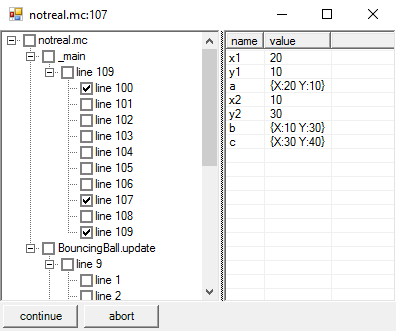
\includegraphics[width=\columnwidth-7pt]{debugger}}

The program will then trigger a breakpoint on the first instruction and launch the debugger GUI.
From the GUI, more breakpoints can be set with the check-boxes.
When the user presses `continue' or `abort', the GUI will close and appear again on the next breakpoint.

The left pane shows a four level deep tree which sorts the program on file name, function name, rule and line.

The right pane shows a table with the name and value of the local identifiers defined up to the current breakpoint.

\subsubsection{Program changes}
When compiling with the debug flag set, some additions are made to target program.

\paragraph{Local identifier table}
After each instruction that defines named local identifiers, a new instruction is generated.

\begin{CS}
    var foo = 42;
    _dbug_symbol_table["foo"] = foo;
\end{CS}

After each assignment to a named local identifier, the named identifier and the value are recorded in a key-value collection. 
This key-value collection will be passed to the debugger when a breakpoint is hit.
A new key-value collection is defined at the start of each rule.

\paragraph{Break points}
When compiling with the debug-flag set, function closures will have a group of static boolean arrays.
One array for each rule in the function.

\begin{CS}[escapeinside=\#\#]
    class #\textit{<function name>}#{
        #\textit{<arguments>}#
        static bool[] _dbug_breakpoints_0;
        static bool[] _dbug_breakpoints_1;
        #\textit{<return value>}# _run(#\textit{<last argument>}#){
            #\textit{<body>}#
        }
    }
\end{CS}

The breakpoints are generated at each line of source code in the rule.
This is different than breaking at every instruction, as normalization often splits single lines into multiple instructions.

\begin{CS}
    ...
    if(_dbug_Breakpoints_1[6]){
        _dbug.breakpoint("filename.mc", 12, 
                         _dbug_symbol_table);
    }
    ...
\end{CS}

\subsubsection{Debug struct}
The breakpoint function is defined as a public static member of the debug struct.

The debugger is defined in a separate file, \verb|_dbug.cs|, which is imported by the target executable.
This is done to keep the program-specific code out of \verb|_dbug.cs|.

\verb|_dbug.cs| contains the struct \verb|_dbug|.
This struct contains only the following public static items.

\begin{enumerate}
    \item the program tree
    \item the breakpoint tree
    \item the breakpoint function
\end{enumerate}

The program builds up the program tree and the breakpoint tree in the main function, before the first user-written line starts.
The trees are both four-levels deep and sorted on filename, function name, rule and line number.
The breakpoint function is called when the program hits a break-point.

This was chosen because breakpoint checks happen every few instructions, so they have a huge effect on debug performance.
Straight arrays with booleans are very fast to index since it only costs one bounds-check, one addition and one dereference.
The dereference can even be done speculatively, due to branch prediction~\cite{branchprediction}.

\paragraph{The tree representation} of the program is four levels deep.
The first level represents the file, the second level represents the function, the third level represents the rule and the fourth level represents the premise.
This tree representation is initialized in the main function, before the user code begins.

\paragraph{The breakpoint table} 
Each closure has its group of breakpoints.
To easily index all the breakpoint arrays from one central point, the \verb|_dbug| struct has a breakpoint table.
The breakpoint table is a static four-dimensional array (\verb|bool[][][][]|) that points to the static breakpoint arrays in the closures.
This way, the arrays are quick to index from the closure, while being available in a tree-like from for the debugger.

\paragraph{The breakpoint function}
The \verb|_dbug| struct contains a static method \verb|breakpoint| that will pause the execution of the program and present the GUI.
When the user presses `continue' or `abort', the GUI will close and the \verb|breakpoint| method will return control back to the program.

The first two arguments to \verb|_dbug.breakpoint| are the filename and the line number to uniquely identify the call site.
The third argument is the symbol table that has been accumulated so far.

\subsubsection{Evolution}
The debugger has changed little, since it is a relatively simple construct.
The only significant changes were the decision to go from a single boolean array per closure to one per rule.
The book-keeping involved in having the boolean arrays packed was inelegant, because there was now a dependency between the rules: the latter breakpoint number depends on the breakpoints in the former rule.


\section{Conclusions}\label{conclusions}
In this thesis, we have shown how typechecked metacasanova can be transformed into an executable program.
We did this by first finding that C\# was the output language of choice.
We then showed a simple interface with an orthogonal IR.
After that, we showed how to map the IR to C\# statements with correctly generated identifiers.
To validate the code generator, a simple interpreter was written, and finally we have shown how to embed a debugger in the executable.

When the back-end was finished, we checked our requirements to see if they have been met.
We showed that the back-end generates correct code and inter-operates with .NET by using test programs that use every IR instruction, including the .NET instructions.
We also showed that the back-end runs on multiple platforms, and that the performance of MC is greater that that of Python with benchmarks.

The result is a working, reliable, performant back-end, with interpreter, validator and embedded debugger.
All finished within the time frame of the internship.

This program, along with the documentation, will help the research group with their implementation of Casanova and the evolution of Meta Casanova.
These technologies can then be applied in the virtual reality and video game development.


% appendix
\setcounter{section}{0}
\renewcommand\thesection{\Alph{section}}
\section{Glossary}
boilerplate code

--- difficult words here ---

\end{multicols}

\printbibliography
\end{document}
